\documentclass{ufabc}

\usepackage{amscd}
\usepackage{amsfonts}
\usepackage{amssymb}
\usepackage{epsf}
\usepackage{graphicx}
\usepackage{algorithm}
\usepackage{algpseudocode}
\usepackage{pifont}
\usepackage{indentfirst}
\usepackage{amsmath}
\usepackage[only,ninrm,elvrm,twlrm,fivrm,sixrm,sevrm,egtrm,egtit,tenrm,tenit,twlit,frtnrm]{rawfonts}

\instituicao{Universidade Federal do ABC\\Centro de Matem�tica, Computa��o e Cogni��o (CMCC)}
\curso{P�s-Gradua��o}{Ci�ncia da Computa��o}{Mestre}
\titulo{Agentes inteligentes para batalhas Pok�mon}
\autor{Jonathan Ohara}{de Araujo}
\orientador{Orientador: Prof. Dr. Fabr�cio Olivetti de Fran�a}
\coordenador{Prof. Dr. Jo�o Paulo G�is}	
\documento{Qualifica��o}
\convidados{Prof. Dr. Fabr�cio Olivetti de Fran�a}{Prof.Dr. Jo�o Paulo Gois}{Prof.Dr. Andr� Luiz Brand�o}{Prof.Dr. Denise Hideko Goya (Suplente)}
	
\date{03}{2016}

% novos comandos para qualificacao
\newcommand{\kCC}{\emph{kCC}}
\newcommand{\kCH} {\emph{kCH}}
\newcommand{\uCC}{\emph{1CC}}
\newcommand{\uCH} {\emph{1CH}}
\newcommand{\dCC}{\emph{2CC}}
\newcommand{\dCH} {\emph{2CH}}
\newcommand{\PTH}{\mathcal{P}}
\newcommand{\Tau}{\mathcal{T}}
\newcommand{\NP}{{\rm NP}}

\begin{document}
	\maketitle

	\pagenumbering{roman}
	
	\begin{resumo}
Esse trabalho explora a cria��o de agentes inteligentes competitivos em um ambiente onde dezenas de milhares de jogadores humanos competem diariamente para melhorar sua coloca��o no sistema de ranqueamento do jogo Pok�mon Showdown.

Escolher o melhor algoritmo e a melhor forma de aprendizado para jogar contra humanos � um dos grandes desafios desse trabalho. Outro importante aspecto que o agente precisa se adaptar � a grande variedade de composi��es de times e Pok�mons que o agente e o seu advers�rio pode montar.

Para obter a melhor flexibilidade o agente ser� submetido somente a batalhas rand�micas onde as composi��o das equipes s�o todas aleat�rias, e a avalia��o de performance do agente ser� feita atrav�s do sistema de ranqueamento do pr�prio jogo.
\end{resumo}
	\begin{resumoingles}

To Do.

\end{resumoingles}

	\tableofcontents
	
	\listoffigures
	
	\listoftables

	\newpage
	
	\pagenumbering{arabic}

	\chapter{Introdu��o}
\label{cap:introducao}

\section{Motiva��o}
\label{sec:motivacao}

Existem diversas finalidades para cria��o de agentes inteligentes para jogos. Podemos enumerar algumas como: adapta��o a diferentes tipos de jogador, gerar diferentes experi�ncias em cada nova partida, gerar grandes desafios entre outras.

Esse trabalho explora a cria��o de agentes inteligentes que compitam com jogadores humanos no sistema de batalhas \textit{Pok�mon} no ambiente \textit{Pok�mon Showdown}.

Um dos grandes desafios na cria��o desses agentes � a adaptabilidade e a competitividade. Diferentes de jogos como xadrez, damas, reversi e outros jogos de tabuleiro, em batalhas \textit{Pok�mon} nada se sabe do advers�rio at� que comece o jogo, ou seja, invalidando qualquer tipo de t�cnica prevendo poss�veis movimentos antes do jogo come�ar j� que cada time pode ser montado de uma infinidade de modos diferentes. Para acentuar ainda mais essas proprieaddes os agentes ir�o treinar e competir no modo rand�mico, nesse modo a escolha do seu time assim como de seu advers�rio � feito pelo pr�prio sistema do jogo.

Por causa da caracter�stica de desconhecimento do time advers�rio, a utiliza��o de t�cnicas de cria��o de �rvores de poss�veis jogadas do advers�rio � bastante prejudicada, pois o agente precisaria predizer os poss�veis \textit{Pok�mons} advers�rios assim como suas caracter�sticas, assim dificultando a utiliza��o da t�cnica que ficou famosa pelo sistema \textit{Deep Blue} que segundo o trabalho \textit{Deep Blue System Overview} \cite{deepblue1} "O \textit{Deep Blue} � um massivo sistema paralelo para realiza��o de busca em �rvores de jogos de xadrez".

\section{Objetivos}
\label{sec:objetivos}
O Objetivo desse trabalho � o desenvolvimento de agentes inteligentes que joguem e aprendam com milhares de jogadores humanos. Ser� implementada distintas t�cnicas para cria��o e aprendizado desses agentes. No decorrer do trabalho ser� sumarizado a evolu��o dos agentes no sistema de ranqueamento do jogo e, essa posi��o ser� confrontada com a quantidade de treinamento que cada agente recebeu, podendo assim observar a curva de melhora em rela��o a quantidade de treinamento.

Para cria��o desses agentes foi desenvolvida uma API (Application Programming Interface) que permitir� a comunica��o com o jogo \textit{Pok�mon Showdown}. Inicialmente a API est� disponibilizada apenas para JavaScript mas durante o desenvolvimento do projeto ser� portada para Java atrav�s de WebSockets.

\section{Principais contribui��es}
\label{sec:principais}

O trabalho ir� explorar a cria��o de agentes inteligentes adaptativos, num ambiente que pouco se sabe sobre o advers�rio. Os agentes ter�o informa��es apenas durante a batalha e, essas informa��es s�o apenas aquelas que o advers�rio realizar. Por exemplo: o agente s� saber� que advers�rio tem um \textit{Pok�mon} at� o mesmo us�-lo, os movimentos que \textit{Pok�mon} tem ser�o apenas conhecidos a medida que o advers�rio utiliz�-los e existem caract�risticas que agente n�o tem como descobrir como por exemplo a quantidade de ataque e defesa distruibida no monstro.

Al�m disso a constru��o de uma API para acesso ao jogo contrubuir� para que outros pesquisadores tamb�m possam desenvolver estudos e criar seus pr�prios agentes podendo criar-se uma cultura de competi��o entre agente inteligentes na plataforma \textit{Pok�mon Showdown}.


	\chapter{Agentes Inteligentes}
\label{cap:agentesInteligentes}

Na computa��o, especialmente em intelig�ncia artificial, � bem comum utilzar-se do termo agente ou agente inteligente. Por defini��o do dicion�rio \cite{michaelis} agente significa "Que age, que exerce alguma a��o; que produz algum efeito".

Na academia temos defini��es mais direcionadas como a de \cite{aiModenApproach} "Um agente � algo capaz de de perceber seu ambiente atrav�s de sensores e agir sobre esse ambiente por meio de atuadores", ou a de \cite{kidsim} "Vamos definir um agente como uma entidade de \textit{software} persistente dedicada para um prop�sito espec�fico. 'Persistente' distingue agentes de sub-rotinas; agentes t�m seus pr�prais ideias sobre como realizar tarefas, suas pr�prias agendas. 'Prop�sitos especiais' os distingue de aplica��es multifuncionais inteiras; agentes s�o tipicamente muito menores."

Existem diversas defini��es de agentes. Mas qual seria a diferen�a de um agente para um programa de computador? Os autores \cite{agentOrProgram} prop�em uma defini��o mais s�lida para agente "Um agente aut�nomo � um sistema situado dentro e como parte de um ambiente que sente esse ambiente e age sobre ele e, ao longo do tempo, busca de sua pr�pria agenda de modo a efetivar o que sente no futuro." ainda segundo os autores maioria dos programas comuns violam uma ou mais regras dessa defini��o, por exemplo um sistema de folha de pagamento sente o ambiente atrav�s de suas entradas e age sobre ele gerando uma sa�da, mas n�o � um agente porque sua sa�da normalmente n�o afeta o que ele sente mais tarde.

\section{Classifica��es de agentes}

Os agentes possuem tamb�m diferentes explica��es quanto a suas caracter�sticas, classifica��es e taxonomia. Uma das defini��es mais antigas e mais s�lidas � a de \cite{Nwana96softwareagents} nesse trabalho o autor define tr�s dimens�es para o agente:

\begin{itemize}

	\item \textbf{Mobilidade}. Capacidade de se mover em torno de alguma rede. Definindo agentes como fixos ou m�veis;
	
	\item \textbf{Deliberativos ou reativos}. Agentes deliberativos possuem simb�los internos, modelos de racioc�nio e se envolvem com o planejamento e negocia��o a fim de conseguir uma coordena��o com outros agentes. J� os reativos agem por est�mulos/respostas que o estado atual do ambiente que est� inserido o proporciona.
	
	\item \textbf{Ideais e atributos prim�rios}. Os agentes podem ser classificados de acordo com tr�s caracter�sticas: autonomia, cooperatividade e aprendizagem. Autonomia se refere ao princ�pio que o agente deve realizar a��es sem interven��o humana. Coopera��o � a habilidade de se comunicar com outros agentes. Aprendizagem � a capacidade de aprender conforme informa��es s�o lidas e a��es sejam realizadas. Dessas defini��es surgem quatro tipos de agentes conforme mostra a Figura \ref{fig:tiposagentes}.
	
\end{itemize}

\begin{figure}[!h]
\centering
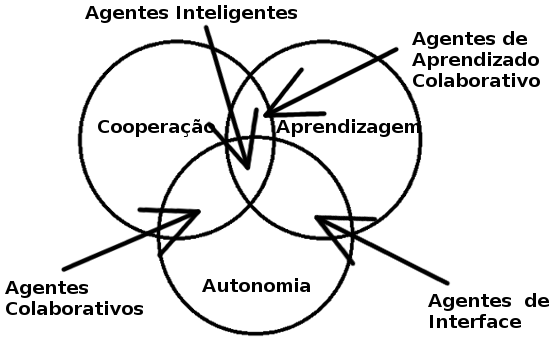
\includegraphics[width=16cm]{figures/tiposagentes.png}
\caption[Vis�o parcial da tipologia de um Agente]{Vis�o parcial da tipologia de um Agente.}
\label{fig:tiposagentes}
\end{figure}

J� \cite{agentOrProgram} classifica os agentes pelas propriedades que eles apresentam, s�o elas: reatividade, autonomia, orienta��o a objetivo, tempor�ria ou cont�nua, comunicativa, aprendizagem, mobilidade, flexibilidade e car�ter.

Emboras as diferentes defini��es, muitas coisas s�o comuns ou muito parecidas como a presen�a de  caracter�sticas como autonomia, aprendizado, objetivos e comunicatividade. 

\section{Agentes em jogos}

Antigamente maioria do processamento do sistema que rodava um jogo(computador, video-game entre outros) era utilizada para processamentos gr�ficos. Com a evolu��o e custo baixo dos equipamentos (\textit{hardware}) hoje em dia � poss�vel dar mais aten��o a outros aspectos de um jogo. O autor \cite{iaInGames} discorre um outro ponto "Como jogos de computador se tornam mais complexos e os consumidores exigem advers�rios mais sofisticados controlados pelo computador, os desenvolvedores de jogos s�o obrigados a colocar uma maior �nfase nos aspectos de intelig�ncia artificial de seus jogos". Por isso hoje, existem um grande n�mero de jogos que n�o s�o conhecidos por sua beleza gr�fica, segundo \cite{aiForGames} um n�mero cada vez maior de jogos tem como principal ponto do jogo a Intelig�ncia Artificial, como por exemplo Creatures[Cyberlife Technology Ltd., 1997] em 1997, e jogos como The Sims[Maxis Software, Inc., 2000] e Black and White [Lionhead Studios Ltd., 2001]. Ainda segundo \cite{aiForGames} o jogo Creatures foi um dos sistemas mais complexos de intelig�ncia artifical visto em um jogo, com um cer�bro baseado em rede neural para cada criatura presente no jogo.

Agentes para jogos tem uma infinidade de pr�positos. Ao associar esses dois termos � bem comum pensar em oponentes controlados por agentes, por�m a utiliza��o de agentes vai muito al�m disso. � poss�vel utiliza��o de agentes em outros aspectos como na gera��o de conte�do procedural, cria��o de desafios e miss�es entre outros.

O artigo \textit{Procedural Content Generation for Games: A survey} \cite{PCGsurvey2013} cita que a gera��o de conte�do atrav�s de agentes inteligentes permite a cria��o de diferentes tipos de terrenos sem perder o controle do \textit{design} do jogo.

O trabalho de \cite{questGenerator2011} explora a gera��o procedural de miss�es e desafio em jogos(especialmente para jogos de MMORPGs \textit{online}), segundo os autores essa abordagem tem o pontencial de aumentar a variedade e a longevidade de um jogo.

Existem tamb�m outras aplica��es para agentes como busca de caminhos em ambientes complexos, gera��o de objetos, danifica��o de objetos entre outras.

\section{Agentes inteligente contra jogadores}

Existem v�rias abordagens para cria��o de agentes que enfrentam jogadores. Pode-se enumerar alguns deles como agentes adaptativos, evolutivos e competitivos.

Em alguns jogos o jogador n�o tem uma op��o de dificuldade, ficando a crit�rio do sistema do jogo controlar a dificuldade, como nos jogos \textit{Middle Earth: Shadow of Mordor} e \textit{Max Payne 2}. Segundo \cite{Ponsen04improvingadaptive} nogo Max Payne 2 � introduzido algo chamado op��es din�micas de dificuldade. Informa��es do mundo do jogo s�o extra�das para estimar a habilidade do jogador, ajustando a dificuldade da intelig�ncia artificial.

Alguns agentes s�o criados para acompanhar a curva de aprendizado de cada pessoa, para que o jogador sempre tenha um bom n�vel de desafio sempre que jogar. No jogo \textit{Star Craft 2} existe o modo chamado pareamento contra Intelig�ncia Artificial, nesse modo o desempenho do jogador em partidas passadas define qual o n�vel do jogador, ou seja, quanto mais o jogador evolui mais dificil ser� seu oponente.

Outra abordagem interessante � a utilizada em Drivatar \cite{microsoft:drivatar} inserida no jogo Forza Motorsport onde o sistema cria agentes "humanizados" que aprendem com a pessoa que est� jogando, incorporando suas caracter�sticas e utilizando para jogar contra o pr�prio jogador. 

Este trabalho explora a cria��o de agentes competitivos, ou seja, agentes projetados para ganhar de jogadores humanos. Segundo \cite{gamesComputerAI1} apenas na d�cada de 90 os computadores foram capazes de competir com sucesso contra o melhor dos humanos. O primeiro jogo a ter um campe�o mundial n�o humano foi o jogo de damas em 1994 seguido pelo Deep Blue em 1997.

O agente jogador mais conhecido � o Deep Blue da IBM. O artigo Deep Blue: System overview \cite{deepblue1} explica o funcionamento do agente. O Deep Blue � composto por um \textit{chip} chamado \textit{Chess Chip} que � dividido em tr�s partes:

\begin{itemize}

	\item \textbf{Buscador alphabeta}. Menor parte do \textit{chip}, contendo apenas 5\% de seu total, esse componente � respons�vel por fazer a busca na �rvore de jogadas. O algoritmo utilizado � uma variante do \textit{alphabeta} chamado de \textit{minimum-window alpha beta search}, essa t�cnica foi escolhida por n�o ser necess�rio uma pilha de valores.
	
	\item \textbf{Gerador de movimentos}. Esse componente cont�m o \textit{array} bidimensional 8x8 referente a cada posi��o do tabuleiro do xadrez, ele tamb�m � respons�vel por realizar e verificar a legalidade dos movimentos de acordo com as regras do xadrez.
	
	\item \textbf{Fun��o de avalia��o}. Ocupando cerca de dois ter�os do \textit{chip} esse componente � respons�vel pela avalia��o dos movimentos. Cada poss�vel posi��o de cada pe�a � avaliado, essa avalia��o � baseada em quatro crit�rios: material, posi��o, seguran�a do rei e tempo \cite{ibmdeepblue}. Material � o quanto cada pe�a "vale". Por exemplo um pe�o vale 1 enquanto uma torre vale 5. Posi��o quantifica o qu�o bom est�o posicionadas as pe�as, nesse c�lculo uma s�rie de aspectos � levado em conta, um deles � o n�mero de movimentos seguros que as pe�as podem fazer para atacar. Seguran�a do rei � calculo que leva em conta a prote��o do rei. Por final tempo, al�m de controlar o tempo da pr�pria jogada, fazer uma jogada r�pida d� ao advers�rio menos tempo para pensar em poss�veis jogadas.
	
\end{itemize}

Como pode ser visto no agente do Deep Blue a heur�stica � algo muito importante na constru��o de um agente para jogos complexos. Em alguns jogos a avalia��o de heur�stica n�o � t�o importante, um exemplo desse tipo de jogo � o jogo da velha pois temos uma �rvore pequena de possibildades e o resultado � vit�ria, empate ou derrota, ou seja, n�o � necess�rio a cada n� da �rvore uma complexa avalia��o de heur�stica.

Segundo \cite{Nielsen:1994:HE:189200.189209} avalia��o heur�stica envolve ter um pequeno conjunto de avaliadores examinando a interface e avaliando a sua conformidade em rela��o ao resultado. 

Os autores \cite{DBLP:conf/aaai/ChristensenK86} dicorrem que, em jogos de tabuleiro de duas pessoas a fun��o de heur�stica � vagamente caracterizado pela "for�a" do posicionamento de um jogador contra o outro. Ainda segundo \cite{DBLP:conf/aaai/ChristensenK86} pode-se dizer que uma fun��o de avalia��o de heur�stica tem duas propriedades:

\begin{itemize}
	\item Quando aplicado a um estado final(no caso de uma �rvore, um n� folha), a avalia��o de heur�stica tem que devolver o estado corretamente;
	\item O valor da fun��o de heur�stica � invari�vel ao longo de um caminho de solu��o �tima.
\end{itemize}

\section{Competi��o de agentes inteligentes}

Um recurso bastante utilizado para pesquisa em intelig�ncia artificial � o desenvolvimento de agentes inteligentes que compitam com outros agentes que utilizem diferentes t�cnicas. Tais competi��es s�o bem comuns nos grandes congressos de intelig�ncia artificial. 

As competi��es de intelig�ncia para Start Craft que ocorrem desde 2010 avan�ou significamente o campo de intelig�ncia artificial para jogos de estrat�gia em tempo real segundo \cite{6637024}. Em Star Craft os jogadores tem que se preocupar em construir um ex�rcito ao mesmo tempo que gere uma economia bem complexa. Nesse jogo o vencedor � definido pelo jogador que derrotar todas as tropas e estruturas advers�rias. Nessa competi��o dois agentes s�o colocados para guerrear at� que haja um vencedor. A comunica��o com o jogo � feito pela BWAPI uma API em C++ que permite comunica��o do agente com o jogo, ou seja, atrav�s dessa biblioteca � poss�vel realizar comandos que ser�o executados no jogo.

A figura \ref{fig:starcraftai} mostra a API funcionando. Ele usa o sistema de conversa do jogo para mostrar mensagens do agente.

\begin{figure}[!h]
\centering
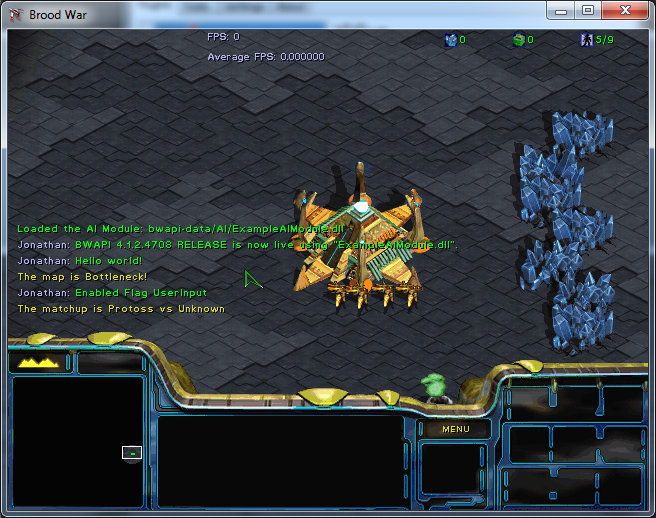
\includegraphics[width=16cm]{figures/bwapi.png}
\caption[BWAPI - StarCraft API]{BWAPI em funcionamento.}
\label{fig:starcraftai}
\end{figure}

Outra competi��o um pouco diferente � a AI Birds \cite{aibirds1}, nessa competi��o os agentes s�o submetidos a jogar Angry Birds, o objetivo desse jogo � voc� destruir objetos(ganhando assim pontos) com pass�ros que s�o arremessados por um estilingue. Diferente do Star Craft nessa competi��o n�o h� um enfretamento direto entre os agentes, eles s�o submetidos a enfrentar o mesmo cen�rio e vence o agente que obtiver mais pontos. A comunica��o com o jogo � bastante diferente do Star Craft, nesse caso o jogo roda via navegador de internet(apenas Google Chrome) e um plugin de JavaScript tira fotos do jogo e passa essa imagem via WebSocket para uma linguagem que ir� interpretar tal foto.

Na figura \ref{fig:angrybirdsai} pode ser visto como a API se comunica com jogo. Uma imagem � caputrada do navegador e a partir disso � utilizado um algoritmo de reconhecimento de imagem para identificar o que � cada coisa(os quadrados em volta do objeto � o que a API est� reconhecendo).

\begin{figure}[!h]
\centering
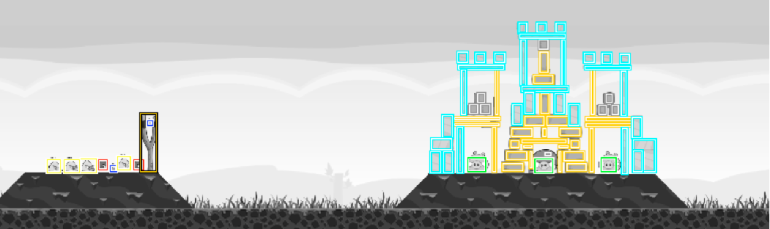
\includegraphics[width=16cm]{figures/aibirds.png}
\caption[AIBIRDS - Angry Birds AI API]{Api Angry Birds AI em funcionamento.}
\label{fig:angrybirdsai}
\end{figure}

%ID�IA: Talvez comentar de outra competi��o como Geometry Friends

Neste trabalho al�m da cria��o de agentes, ser� explorado a cria��o de uma API para comunica��o com o jogo Pok�mon Showdown que � um simulador de batalhas Pok�mon. No cap�tulo \ref{cap:batalhasPokemon} ser� explicado como funciona o sitema de batalhas. A API possibilita batlahas contra outros agentes e contra jogadores humanos. A API est� escrita em JavaScript mas tamb�m haver� possiblidade de comunica��o via WebSocket onde qualquer linguagem que tenha o recurso pode fazer um agente.
	\chapter{Intelig�ncia Artificial}
\label{cap:inteligenciaArtificial}

Neste cap�tulo � feito uma revis�o das t�cinicas de intelig�ncia artificial que ser�o utilizadas nesse trabalho. Algoritmos baseados em grafos \ref{sec:algoritmoGrafos}, aprendizado por refor�o \ref{sec:aprendizadoReforco} e neuroevolu��o \ref{sec:neuroevolucao}.

\section{Intelig�ncia para jogos}
\label{sec:inteligenciaJogos}

O estudo de IA/IC (Intelig�ncia artificial/Intelig�ncia computacional) para jogos � uma �rea de estudo que vem crescendo muito na �ltima d�cada. Grandes confer�ncias como o IEEE Conference on Computational Intelligence and Games (CIG), AAAI Aritificial Intelligence and Interactive Digital Entertainment (AIIDE) e IEEE Transactions on Computational Intelligence and AI in Games (TCAIG) j� contam com mais de dez edi��es.

Jogos podem ser usados como cen�rio desafiador para avalia��o de m�todos de intelig�ncia computacional, pois eles prov�m elementos din�micos e competitivos que s�o pertinentes ao mundo real \cite{cig2014}.

Segundo \cite{panoramaAIGames} durante so semin�rios em Dagstuhl(centro de pesquisa de ci�ncia da computa��o alemanha) foi poss�vel identificar dez grandes t�picos em IA/AC:

\begin{itemize}
	\item  Aprendizado de comportamento para jogadores n�o humanos (JNH); 
	\item  Busca e planejamento;
	\item  Modelagem de personagens;
	\item  Jogos como avalia��o comparativa para Intelig�ncia Artificial (IA);
	\item  Gera��o de conte�do procedural;
	\item  Narrativa computacional;
	\item  Agentes cr�veis;
	\item  \textit{Game design} assistido por IA;
	\item  IA para jogos em geral;
	\item  IA em jogos comerciais.
\end{itemize}

Ainda segundo \cite{panoramaAIGames} todas as �reas de pesquisa podem ser vistas como potenciais influenciadores delas mesmas em algum grau. Essas conex�es e interconex�es geram outras �reas de pesquisa.

Nas pr�ximas se��es ser� feito uma revis�o dos principais m�todos que � utilizado nos jogos e que ser�o usados neste trabalho.

\section{Algoritmos baseados em grafos}
\label{sec:algoritmoGrafos}

Um dos grandes desafios de um  agente e de um jogador dentro de um jogo � a tomada de decis�o, expandindo um pouco essa ideia, pode-se dividir a tomada de decis�o em partes menores: levantar op��es, avaliar as op��es e escolher qual pode conduzir o jogador a vit�ria dado um determinado cen�rio.

Uma algoritmo muito comum para esse cen�rio � o \textit{minimax}. Segundo \cite{browne12asurvey} jogos do mundo real normalmente envolvem uma estrutura de recompensas em que apenas as recompensas obtidas em estados terminais(jogadas que definem quem � o vencedor) do jogo descrevem com precis�o o qu�o bem cada jogador est� se saindo. Os jogos s�o, portanto, normalmente modelado como �rvores de decis�es da seguinte forma:

\begin{itemize}
	
	\item \textbf{Minimax} tenta minimizar recompensa m�xima do oponente em cada estado, e � a abordagem tradicional para pesquisa de jogos combinat�rios em dois jogadores.
	
	\item \textbf{Expectimax} generaliza \textit{minimax} para jogos estoc�sticos em que as transi��es de estado para estado s�o probabil�stica. O valor de um n� � a soma dos valores dos n�s filhos ponderados por suas probabilidades(possibilidade de um estado ocorrer). Estrat�gias de poda de �rvore mais complexas devido a probabildade de um n� acontecer.

	\item \textbf{Miximax} � semelhante ao \textit{expectimax} de apenas um jogador e � usado principalmente em jogos com informa��es n�o precisas. Ele usa uma estrat�gia  predefinida para tratar a decis�o do oponente como n�s probabil�sticos.
	
\end{itemize}

O trabalho de \cite{campbell1983comparison} descreve o algoritmo de \textit{minimax} do seguinte modo: O algoritmo assume que existem dois jogadores chamados Max e Min, e atribui um valor para cada n� dentro da �rvore(de decis�o) do jogo(e tamb�m para n� raiz) do seguinte modo: N�s folhas ou terminais podem dar o valor \textit{minimax} recursivamente. Se a jogada p do jogador Max for escolhida, ent�o o valor de p � o m�ximo valor dos filhos de p. Similarmente, se for a vez do jogador Min ser� escolhido o menor valor dos sucessores de p.  

Na figura \ref{fig:minimaxjogodavelha} � mostrado a aplica��o do algoritmo de \textit{minimax} para um cen�rio do jogo da velha. Na imagem o jogador Max � representado pelo caractere \textbf{X} e o jogador Min por \textbf{O}. Como dito anteriormente a an�lise dessa �rvore come�ou a ser feita pelos n�s terminais, em situa��es vit�riosas foi atribu�do o valor de 10, em empates 0 e em derrota o valor -10. Em seguida, os pai desses n�s folhas s�o preenchidos com o m�nimo ou o m�ximo valor dos n�s filhos. No primeiro n� de MIN(primeiro n� da segunda fileira) existem dois n�s filhos, um com valor 10 e outro com valor -10, por ser um n� MIN � atribuido para esse n� o menor valor(no caso -10). A linha em azul mostra a melhor jogada no momento para o n� raiz.

\begin{figure}[!h]
\centering
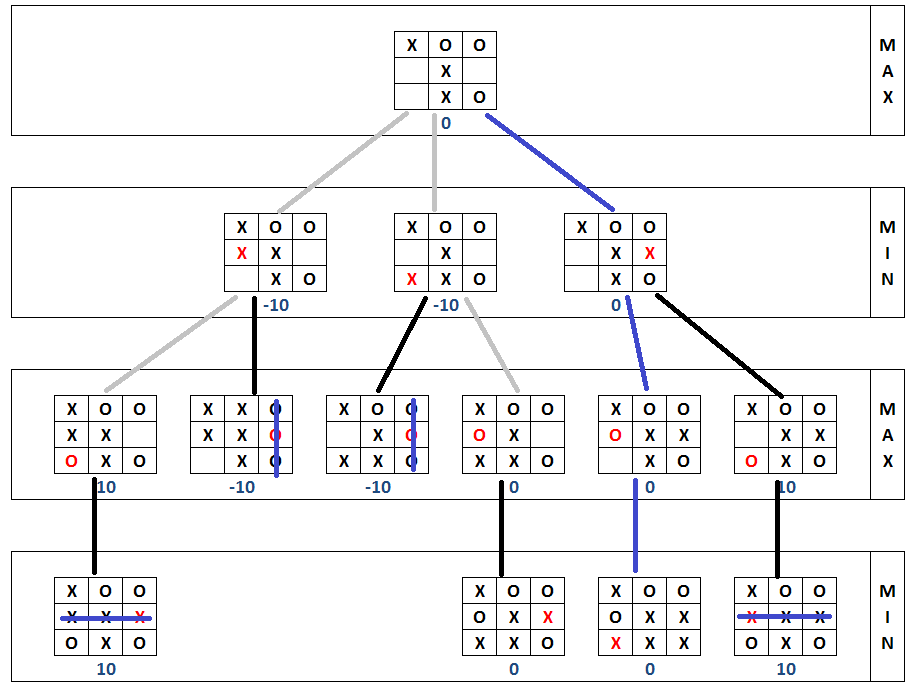
\includegraphics[width=16cm]{figures/minimax.png}
\caption[Minimax]{\textit{Minimax} aplicado a um cen�rio de jogo da velha.}
\label{fig:minimaxjogodavelha}
\end{figure}

Repare que a melhor jogada indicada pelo algoritmo gera um empate. Segundo \cite{evoltuinaryneuralnetworks} um dos problemas do \textit{minimax} � presumir que sempre o advers�rio ir� fazer a melhor escolha poss�vel. Muitas vezes, em situa��es de derrota iminente a melhor jogada pode n�o ser para o mais alto de \textit{minimax}, especialmente se ele ainda ir� resultar em uma derrota.

Outro problema do \textit{minimax} � a quantidade de n�s que ele precisa analisar em jogos com grande n�mero de poss�veis jogadas e que duram um grande n�mero de turnos(grande profundidade na �rvore). Uma t�cnica muito utilizada para mitigar esse problema � a chamada poda \textit{alpha-beta}.

Segundo \cite{knuth1976analysis} essa � tecnica � usada geralmente para aumentar a velocidade de busca sem perder informa��o. Nessa t�cnica s�o ignorado n�s e suas sub-�rvores de jogadas incapazes de ser melhor que movimentos que j� conhecemos. Durante a an�lise das jogadas s�o definidas duas v�riaveis \textit{alpha} e \textit{beta}. \textit{Alpha} representa o valor m�ximo que o jogador Max e \textit{beta} a pontua��o m�nima  do jogador Min. A cada avalia��o de n� esses limites s�o verificados, caso o valor da avalia��o n�o estiver entre esses limites o n� e todas suas �rvores s�o cortados.

Outra t�cnica de otimiza��o do \textit{minimax} � a �rvore de Busca de Monte Carlo(MCTS). Segundo \cite{campbell1983comparison} o processo de construn��o da MCTS � feita de modo incremental e assim�trico na forma: para cada itera��o do algoritmo, uma "pol�tica de �rvore"  � utilizada para definir o n� mais urgente da �rvore atual. A pol�tica da �rvore tenta balancear considera��es da explora��o(procura areas que aindan�o tenham sido bem amostradas) e explora��o(procura areas que parecem ser promissoras). O n� escolhido � avaliado e todos seus ancetrais s�o atualizados com suas novas estat�sticas.

Uma das grandes vantagens do MCTS � a possibilidade de utilizar de maneira incremental, ou seja, � poss�vel delimitar um tempo ou n�mero m�ximo de itera��es que o algoritmo ir� rodar, facilitando a aplica��o em ambientes que exigem baixo tempo de resposta(jogos de tempo real) ou tempo de respsota fixado(jogos baseados em turno).

\section{Aprendizado por refor�o}
\label{sec:aprendizadoReforco}

Uma t�cnica bastante utilizada em aprendizado de m�quina � o aprendizado por refor�o (RL). Segundo \cite{Sutton:1998:IRL:551283} a ideia de aprender interagindo com nosso ambiente provavelmente � a primeira coisa que nos ocorre quando pensamenos sobre aprendizado natural.

Segundo \cite{kaelbling1996reinforcement} o algoritmo de aprendizado por refor�o � um 	modo de programar agentes por um sistema de puni��o e recompensa sem precisar especificar como a tarefa precisa ser realizada.

Segundo \cite{Mitchell:1997:ML:541177} o aprendizado por refor�o pode resolver tarefas como aprender a controlar um rob� m�vel, aprender a otimizar opera��es em f�bricas, e aprender a jogar jogos de tabuleiros.

Novamente segundo \cite{kaelbling1996reinforcement} existem duas principais estrat�gias para resolver problemas com aprendizado por refor�o. A primeira � uma busca entre os poss�veis comportamentos para achar aquele que se adequa bem ao ambiente. O Segundo modo � utilizar m�todos estoc�sticos e m�todos de programa��o din�mica para estimar a utilidade de tomar a��es em estados do mundo.

A figura a \ref{fig:aprendizadoporreforco} mostra o funcionamento b�sico do algoritmo. O agente est� em um determinado estado e executa uma a��o recebendo uma recompensa ou puni��o e vai para um novo estado.

\begin{figure}[!h]
\centering
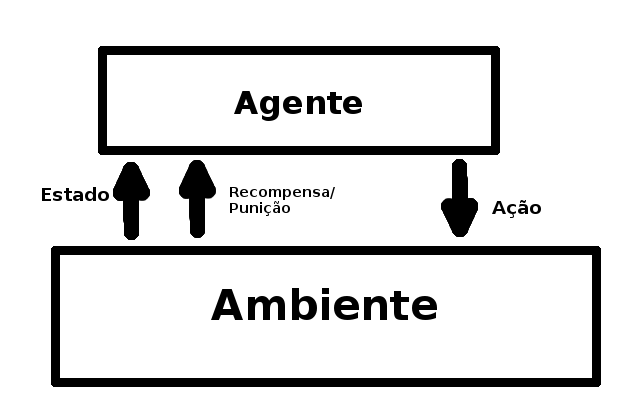
\includegraphics[width=16cm]{figures/basicrl.png}
\caption[Funcionamento aprendizado por refor�o]{Esquema padr�o do aprendizado por refor�o.}
\label{fig:aprendizadoporreforco}
\end{figure}

Existe uma s�rie de altera��es nessa abordagem para abrangir uma maior gama de problemas. Uma varia��o bem comum � a situa��o chamada de recompensa atrasada. Segundo \cite{Mitchell:1997:ML:541177} existe alguns aspectos diferentes ao considerar utilizar aprendizado por refor�o para alguns problemas:

\begin{itemize}
	
	\item \textbf{Recompensa atrasada}. Grandes recompensas podem estar somente em estados que ser�o apenas alcan�ados num futuro long�nquo.
	
	\item \textbf{Explora��o}. No aprendizado por refor�o, o agente influencia a distribui��o do treino pela sequ�ncia de a��es qe escolhe. Com isso surge a d�vida qual das estrat�gias produz o mais efetivo aprendizado (para colher novas informa��es). Explorar todos as poss�veis a��es, ou explorar estados e ac�es j� conhecidos com alta recompensa (para maximizar a sua recompensa culmulativa).

	\item \textbf{Estados parcialmente observ�veis}. Em muitos casos os sensores do agente n�o consegue observar o estado inteiro do ambiente. Por exemplo, um rob� com c�mera frontal n�o pode enxegar o ambiente que est� atr�s dele.
	
	\item \textbf{Aprendizagem ao longo da vida}. Possibilidade de utilizar conhecimentos obtidos anteriormentes para reduzir a complexidade de aprender novas Tarefas.
	
\end{itemize}

Uma das t�cnicas que resolve esse problema � a chamada processo de decis�o de Markov(MDP). Segundo \cite{kaelbling1996reinforcement} consiste em:

\begin{itemize}
	
	\item Um conjunto de estados chamado S,
	\item Um conjunto de a��es chamado A,
	\item Uma fun��o de recompensa onde $R: S\times A \rightarrow \mathbb{R}$,
	\item Uma fun��o de transi��o entre o estados onde $T: S\times A \rightarrow II(S)$.
	
\end{itemize}

A fun��o de transi��o de estados espec�fica o pr�ximo estado como uma fun��o do estado atual e a a��o do agente. Para que isso seja v�lido o ambiente tem que satisfazer a propridade de Markov, que diz que a transi��o de estados tem que ser independente de qualquer informa��o de estados e a��es do agentes anteriores.

Com essas propriedades � poss�vel calcular qualquer estado futuro pela fun��o de transi��o de estados resolvendo o problema de recompensa atrasada, como � poss�vel calcular todos os poss�veis futuros e estados e a��es tamb�m � poss�vel calcular futuras recompensas.


\section{Neuroevolu��o}
\label{sec:neuroevolucao}
	\chapter{Sistemas de batalhas Pok�mon}
\label{cap:batalhasPokemon}

Esse cap�tulo apresentar� o sistemas de batalhas dos jogos \textit{Pok�mon}. Como dito nos cap�tulos anteriores � preciso conhecer bem o ambiente que o agente est� inserido para poder aferir avalia��es e tomar decis�es. Este cap�tulo est� organizado da seguinte maneira: na se��o \ref{sec:contextualizacaopokemon} � feita uma breve contextualiza��o sobre o jogo e a franquia \textit{Pok�mon}. Na se��o \ref{sec:ambientepokemonshowdown} � apresentado o simulador \textit{on-line} de batalhas chamado de \textit{Pok�mon Showdown!}. No cap�tulo \ref{sec:batalhaspokemon} ser� explicado como funciona o sistema de batalha.

\section{Contextualiza��o}
\label{sec:contextualizacaopokemon}

Segundo \cite{7336034} \textit{Pocket Monsters} ou Pok�mon � uma s�rie de jogos desenvolvida pela \textit{Game Freak and Creatures Inc.} e publicada pela Nintendo como parte da franquia Pok�mon. O primeiro lan�amento foi em 1996 no Jap�o para o console Game Boy Color, a principal s�rie do jogo � baseada em \textit{Role-Playing-Game} (RPG) e continua a ser lan�ado para consoles port�teis at� hoje.

Ainda segundo \cite{7336034} o objetivo dos jogos de RPG de Pok�mon � capturar monstros chamados de Pok�mon e com eles conseguir ganhar ins�gnias de gin�sios (pr�mio dado por vencer o l�der de gin�sio em uma batalha Pok�mon), para assim ter acesso a liga Pok�mon e se tornar o campe�o dessa (torneio com os melhores treinadores Pok�mon do jogo).

\section{Pok�mon Showdown!}
\label{sec:ambientepokemonshowdown}

Pok�mon Showdown � um simulador de batalhas Pok�mon. Permitindo jogar batalhas \textit{online}! Jogar com times gerados aleatoriamente, ou construindo seu pr�prio time (\cite{pokemonshowdown1}).

Esse ambiente � totalmente \textit{on-line} e pode ser jogado via navegador de internet. O c�digo fonte do jogo � disponibilizado sobre a licen�a MIT. O dono e principal mantenedor do projeto � Guangcong Luo e todo c�digo fonte do projeto pode ser encontrado no Git Hub.

O ambiente conta um grande n�mero de jogadores simult�neos. Durante o desenvolvimento do trabalho foi verificado que muitas vezes o n�mero de usu�rios simult�neos ultrapassou a quantidade de 10.000.

O modo de batalha utilizado durante esse trabalho � o \textit{Random battle} onde o jogo procura um jogador oponente para batalhar e d� para ambos, times aleat�rios.

\section{Batalhas}
\label{sec:batalhaspokemon}

Para poder entender como funciona a mec�nica dos jogos Pok�mon � preciso apresentar todos os elementos que fazem parte do sistema de batalha.

\subsection{Caracter�sticas Pok�mon}

Atualmente existem mais de 720 esp�cies de Pok�mons diferentes dispon�veis no jogo. As principais caracter�sticas dos Pok�mons s�o:

\begin{itemize}
	\item \textbf{Esp�cie}. Nome do Pok�mon (Bulbasaur, Charmander, Squirtle e etc);
	\item \textbf{Tipo}. Um Pok�mon pode ter um ou dois tipos diferentes;
	\item \textbf{G�nero}. Um Pok�mon pode macho, f�mea ou sem g�nero;
	\item \textbf{Peso}. Peso do Pok�mon;
	\item \textbf{Estat�sticas base}. As estat�stica ou atributos s�o separado em 6 categorias:
		\subitem \textbf{HP ou PV} Quantidade de pontos de vida Pok�mon;
		\subitem \textbf{Attack ou Ataque} Quantidade de ataque f�sico do Pok�mon;
		\subitem \textbf{Defense ou Defesa} Quantidade de defesa f�sica do Pok�mon;
		\subitem \textbf{Special Attack ou Ataque Especial} Quantidade de ataque m�gico do Pok�mon;
		\subitem \textbf{Special Deffense ou Defesa Especial} Quantidade de defesa m�gica do Pok�mon;
		\subitem \textbf{Speed ou Velocidade} Velocidade do Pok�mon;
	\item \textbf{Habilidades}. Um Pok�mon tem uma habilidade especial (muitas vezes o que diferencia 2 Pok�mons do mesmo tipo al�m das estat�sticas base, s�o suas poss�veis habilidades);
\end{itemize}

Para calcular a estat�stica real do Pok�mon alguns outros atributos s�o necess�rios. Esses atributos s�o definidos pelo jogador (com exce��o do n�vel que � definido pelo Pok�mon Showdown em alguns modos de jogo):

\begin{itemize}
	\item \textbf{Level}. N�vel do Pok�mon. Onde $0 \leq level \leq 100$.
	\item \textbf{Effort Values ou EV}. Valores de esfor�o, cada Pok�mon tem 510 pontos de EV que podem ser distribu�dos em qualquer um dos 6 atributos, com a limita��o de que cada atributo pode ter no m�ximo 252 pontos de EV.
	\item \textbf{Individual Values ou IV}. Valores individuais, cada estat�stica do Pok�mon tem um valor de IV associado que varia entre 0 e 31. No ambiente Pok�mon Showdown todos os Pok�mons est�o com 31 de IV para todos os 6 atributos.
	\item \textbf{Nature}. Natureza do Pok�mon. Existem 25 diferentes naturezas que um Pok�mon pode ter, sendo que 21 delas alteram atributos. As naturezas que alteram atributos adicionam 10\% em um determinado atributo e reduzem 10\% em outro atributo. A tabela \ref{table:tabelaNatureza} mostra as poss�veis naturezas e as modifica��es dos atributos.
\end{itemize}

\begin{table}[]
\centering
\caption{Naturezas do Pok�mon}
\label{table:tabelaNatureza}
\begin{tabular}{|c|c|c|}
\hline
\textbf{Natureza} & \textbf{Atributo aumentado} & \textbf{Atributo diminu�do} \\ \hline
Lonely            & Ataque                      & Defesa                      \\ \hline
Brave             & Ataque                      & Velocidade                  \\ \hline
Adamant           & Ataque                      & Ataque Especial             \\ \hline
Naughty           & Ataque                      & Defesa Especial             \\ \hline
Bold              & Defesa                      & Ataque                      \\ \hline
Relaxed           & Defesa                      & Velocidade                  \\ \hline
Impish            & Defesa                      & Ataque Especial             \\ \hline
Lax               & Defesa                      & Defesa Especial             \\ \hline
Modest            & Ataque Especial             & Ataque                      \\ \hline
Mild              & Ataque Especial             & Defesa                      \\ \hline
Quiet             & Ataque Especial             & Velocidade                  \\ \hline
Rash              & Ataque Especial             & Defesa Especial             \\ \hline
Calm              & Defesa Especial             & Ataque                      \\ \hline
Gentle            & Defesa Especial             & Defesa                      \\ \hline
Sassy             & Defesa Especial             & Velocidade                  \\ \hline
Careful           & Defesa Especial             & Ataque Especial             \\ \hline
Timid             & Velocidade                  & Ataque                      \\ \hline
Hasty             & Velocidade                  & Defesa                      \\ \hline
Jolly             & Velocidade                  & Ataque Especial             \\ \hline
Naive             & Velocidade                  & Defesa Especial             \\ \hline
Hardy             & Nenhum                      & Nenhum                      \\ \hline
Docile            & Nenhum                      & Nenhum                      \\ \hline
Serious           & Nenhum                      & Nenhum                      \\ \hline
Bashful           & Nenhum                      & Nenhum                      \\ \hline
Quirky            & Nenhum                      & Nenhum                      \\ \hline
\end{tabular}
\end{table}

Finalmente o c�lculo da estat�stica atual � dado pela seguinte equa��o:

\begin{equation}
V = \Bigg( \frac{ \Big( ( 2 \times Base + IV + \frac{EV}{4} ) \times level \Big) }{100} + 5 \Bigg) \times Nature
\end{equation}

Essa equa��o vale para todos os atributos menos para o atributo HP. A Equa��o do HP tem uma pequena modifica��o que � mostrada na equa��o a seguir:

\begin{equation}
V = \Bigg( \frac{ \Big( ( 2 \times Base + IV + \frac{EV}{4} ) \times level \Big) }{100} + level + 10 \Bigg)
\end{equation}

Onde:

\begin{itemize}
	\item \textbf{V} � o valor final, valor que o jogador ir� ver no jogo.
	\item \textbf{Base} � a quantidade b�sica da estat�stica.
	\item \textbf{Nature} Se a natureza do Pok�mon favorecer esse atributo o valor � atribu�do 1.1, caso a natureza desfavore�a esse valor � 0.9 e caso a natureza n�o influa nesse atributo o valor � 1.
\end{itemize}

EVs, IVs e Natureza do Pok�mon s�o importantes customiza��es que fazem um Pok�mon ser diferente de outro, mesmo eles sendo da mesma esp�cie. Na batalha esses 3 valores n�o est�o dispon�veis para o seu advers�rio. 

Para exemplificar e mostrar a diferen�a que a distribui��o de valores pode causar, a seguir ser� calculado o atributo "Especial Ataque"  para 2 Pok�mons da esp�cie Mewtwo ambos no n�vel 100. O Pok�mon Mewtwo tem 154 pontos de Ataque Especial base.

O primeiro Mewtwo ser� chamado de Mewtwo A. O Mewtwo A � da natureza Modest e tem 252 pontos de EV em Ataque Especial e 31 pontos de IV no atributo Ataque Especial. Substituindo essas vari�veis na equa��o:

\begin{equation}
447.7 = \Bigg( \frac{ \Big( ( 2 \times 154 + 31 + \frac{252}{4} ) \times 100 \Big) }{100} + 5 \Bigg) \times 1.1
\end{equation}

O segundo Mewtwo ser� chamado de Mewtwo B. O Mewtwo B � da natureza Adamant e tem 0 pontos de EV em Ataque Especial e 0 pontos de IV no atributo Ataque Especial. Substituindo essas vari�veis na equa��o:

\begin{equation}
281.7 = \Bigg( \frac{ \Big( ( 2 \times 154 + 0 + \frac{0}{4} ) \times 100 \Big) }{100} + 5 \Bigg) \times 0.9
\end{equation}

A diferen�a do atributo Especial Ataque do Mewtwo A e do Mewtwo B � de 166 pontos, ou seja, o Mewtwo A tem cerca de 66\% mais pontos nesse atributo que o Mewtwo B. 

\subsubsection{Habilidades, itens e golpes dos Pok�mons}

Esses 3 aspectos s�o importantes na customiza��o do Pok�mon, pois al�m de ter uma grande variedade de op��es, tais aspectos n�o s�o vis�veis para o seu oponente.

Habilidades s�o efeitos passivos que podem ajudar dentro de batalha. Pok�mons tem entre 1 e 3 poss�veis habilidades podendo escolher apenas 1 delas (ficando a cargo do jogador qual escolher). Existem cerca de 200 habilidades diferentes. Um exemplo de habilidade � a \textit{Intimidate}, quando um Pok�mon com a habilidade \textit{Intimidate} entra em batalha o Pok�mon advers�rio tem seu ataque reduzido em 50\%.

Cada Pok�mon pode carregar consigo um item, esse item tamb�m traz certos tipos de benef�cios para o Pok�mon. Alguns itens s�o ativados quando uma condi��o ocorre na batalha, outros itens s�o cont�nuos. Existem cerca de 300 itens diferentes. Um exemplo de item � o \textit{Leftovers} que recupera $\frac{1}{16}$ do HP total do Pok�mon ao final de cada turno.

Uma das customiza��es mais importantes � quais golpes o Pok�mon ir� poder utilizar. Cada Pok�mon pode escolher 4 golpes entre dezenas de golpes dispon�veis. Cada esp�cie de Pok�mon pode aprender um conjunto diferente de habilidades dependendo do seu tipo e caracter�sticas (por exemplo, apenas Pok�mons com chifre conseguem aprender o golpe Mega Horn). Existem cerca de 600 golpes diferentes.

As principais caracter�sticas dos golpes s�o:

\begin{itemize}
	\item \textbf{Base Power ou Base de For�a}. A for�a base utilizada no c�lculo de dano.
	\item \textbf{Category ou Categoria}. Existem tr�s tipos de categorias:
		\subitem \textbf{Status ou Condi��o} Golpes que n�o infringem dano diretamente, por�m tem algum efeito com grande chance de sucesso para compensar.
		\subitem \textbf{Physical ou F�sico} Golpes f�sicos utilizam o Ataque para c�lculo de dano e Defesa para c�lculo da resist�ncia.
		\subitem \textbf{Special ou Especial} Golpes especiais utilizam o Ataque Especial para c�lculo de dano e Defesa Especial para c�lculo da resist�ncia.
	\item \textbf{Tipo}. Se o tipo do golpe for um dos tipos do Pok�mon a base de for�a � aumentada em 50\% (fen�meno chamado de STAB ou \textit{Same Type Attack Bonus}).
	\item \textbf{Accuracy ou Precis�o}. A chance em percentagem de um golpe acertar.
	\item \textbf{PP ou Pontos de Poder}. A quantidade de vezes que um Pok�mon pode usar um golpe durante uma batalha.
	\item \textbf{Efeito Secund�rio}. Um golpe pode ter um efeito secund�rio, esse efeito tem uma chance de acontecer e pode afetar uma s�rie de coisas como, por exemplo, deixar o oponente paralisado ou aumentar algum atributo.
\end{itemize}

\subsection{Composi��o dos times}

Os dois modos de batalhas mais jogados do Pok�mon Showdown s�o: Random Battles e OU Battles. Em ambos os modos cada time conta com 6 Pok�mons (grande maioria dos tipos de jogos utilizam 6 Pok�mons para compor um time).

Para entender melhor esses 2 modos � preciso entender algumas defini��es do Pok�mon competitivo.

Existe uma comunidade chamada Smogon \cite{smogon}, essa comunidade regula e define as regras que s�o utilizadas em cada modo de jogo, para que o jogo se torne mais competitivo e balanceado. Um dos principais trabalhos da Smogon � balancear os mais de 720 Pok�mons distribuindo eles em faixas chamadas de \textit{tiers}. Do mais fraco para o mais fortes os principais \textit{tiers} s�o:

\begin{itemize}
	\item \textit{Never Used} ou NU;
	\item \textit{Rarely Used} ou RU;
	\item \textit{Under Used} ou UU;
	\item \textit{Over Used} ou OU;
	\item \textit{Ubers}.
\end{itemize}

No modo OU Battles como o pr�prio nome sugere o jogador pode montar seu time com qualquer Pok�mon do \textit{tier} OU e de \textit{tiers} inferiores, nesse modo todos os Pok�mons se enfrentar�o no mesmo n�vel.

Em batalhas rand�micas, para balancear os Pok�mons de diferentes \textit{tiers} � atribu�do diferentes n�veis de acordo com o \textit{tier} do Pok�mon. Pok�mons NU batalham no n�vel 86, RU 82, UU 78, OU 74, \textit{Ubers} 70.

Em cada diferente modo de jogo o jogador tem sua pontua��o de \textbf{Elo} que � uma pontua��o no ranquemanto geral do jogo. Em cada jogo o jogador ganha ou perde pontos de Elo de acordo com o resultado da partida. A quantidade de pontua��o ganha � feita pela diferen�a do seu Elo para o advers�rio. O jogo sempre tenta parear jogadores com pontua��o de Elo semelhante.

Por padr�o cada jogador inicia com 1000 pontos de Elo. Em batalhas com n�veis parecidos de Elo � comum ganhar/perder 20 pontos por partida. Atualmente os jogadores que lideram as coloca��es do modo Random Battle t�m cerca de 2.200 pontos.

\subsection{Sistema de batalhas}

Nessa subse��o ser�o apresentados os principais aspectos de uma batalha, estes aspectos s�o vitais para constru��o dos agentes, pois � baseado nesses pontos que as decis�es ser�o tomadas.

O sistema de batalhas � baseado em dois jogadores em um sistema de turno, ou seja, a cada come�o de turno, cada jogador escolhe qual a��o ir� tomar.

No modo Random Battles um de seus Pok�mons � escolhido aleatoriamente para come�ar a batalha. Em modos como OU Battles � poss�vel escolher qual ser� o primeiro Pok�mon em campo. Os Pok�mons colocados em primeiro na batalha s�o chamados de \textit{lead} e s�o uma pe�a muito importante para o time.

Em situa��es normais, cada turno o jogador pode escolher duas grandes a��es. A primeira � utilizar um dos quatro golpes do Pok�mon. A segunda � trocar o Pok�mon em campo para outro Pok�mon desde que ele esteja vivo. Ao trocar de Pok�mon voc� perde o seu turno, ou seja, logo que o Pok�mon escolhido entrar em batalha ele tomar� o golpe que o advers�rio escolheu no in�cio de seu turno (caso o oponente n�o tenha escolhida trocar de Pok�mon).

Uma das primeiras situa��es onde os atributos do Pok�mon s�o relevantes � para definir quem ser� o primeiro Pok�mon a atacar. Em situa��es normais o primeiro Pok�mon que ataca � aquele com Velocidade entre os dois.

\subsubsection{Sistema de vantagens de tipos}

Alguns tipos de Pok�mons tem vantagem sobre outros tipos de Pok�mons. A ideia � baseada no sistema papel pedra tesoura, onde o papel ganha de pedra, pedra ganha de tesoura e por sua vez tesoura ganha de papel.

Por�m no sistema de batalhas Pok�mon essa mec�nica � um pouco mais complexa. Al�m de existir 18 tipos diferentes de Pok�mon, um Pok�mon pode ter dois tipos distintos.

A imagem a seguir foi retirada do site \cite{bulbapedia1} e cont�m uma tabela mostrando o modificador de dano para cada tipo de golpe em rela��o ao tipo do advers�rio. Ao escolher um golpe, o tipo (golpes tem apenas um �nico tipo) desse golpe � confrontado nessa tabela de acordo com o tipo do advers�rio, caso o advers�rio tenha dois tipos a consulta nessa tabela � feita duas vezes e os modificadores s�o multiplicados gerando um modificar final.

\begin{figure}[!h]
\centering
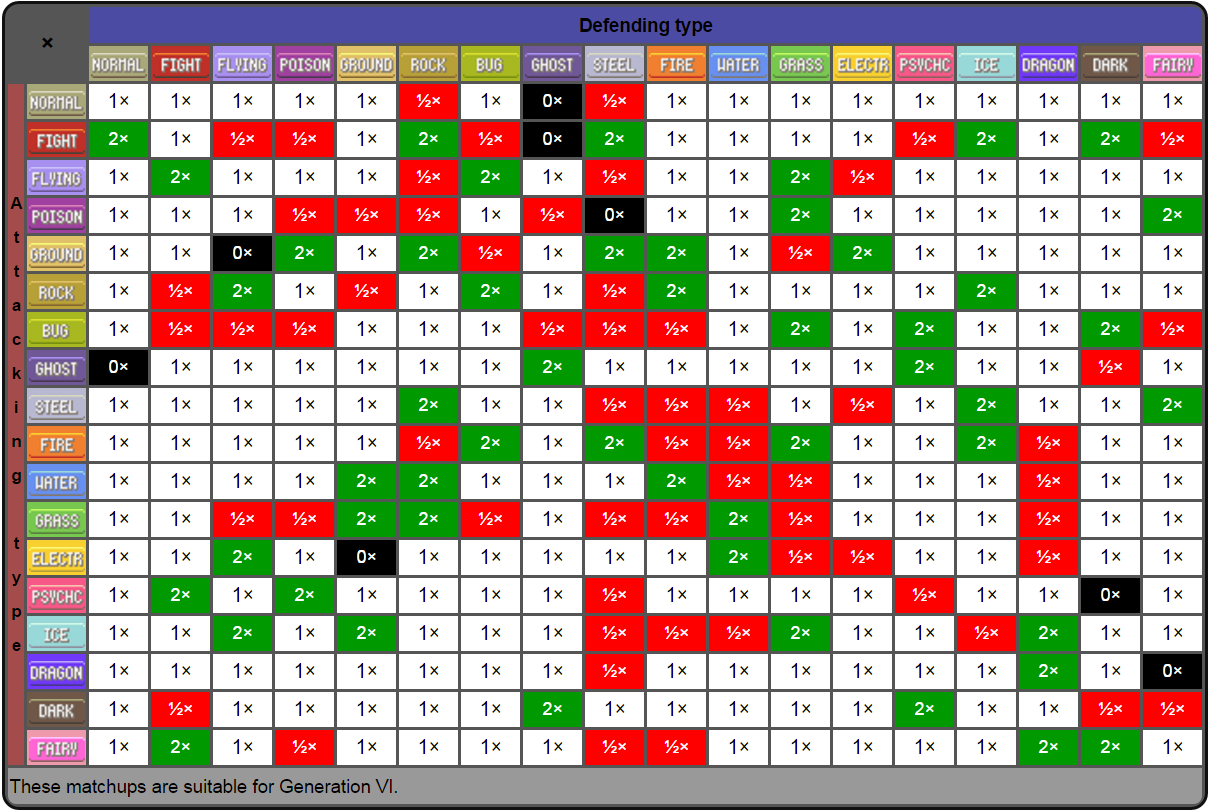
\includegraphics[width=16cm]{figures/pokemontypechart.png}
\caption[Tabela de vantagens e desvantagens do Pok�mon]{Tabela de vantagens e desvantagens do Pok�mon. \cite{bulbapedia1}}
\label{fig:pokemontypechart}
\end{figure}

\subsubsection{Sistema de c�lculo de dano}

Para calcular a quantidade de HP que um Pok�mon ir� perder � utilizada a seguinte equa��o:

\begin{equation}
Dano = \Bigg( \frac{ 2 \times Level + 10 }{ 250 } \times \frac{Attack}{Defense} \times Base + 2 \Bigg) \times Modifier
\end{equation}

Onde:
\begin{itemize}
	\item \textbf{Dano}. Quantidade de dano que o Pok�mon ir� receber.
	\item \textbf{Attack}. � quantidade de Ataque caso o golpe seja da categoria f�sico, ou quantidade Ataque Especial caso o golpe seja da categoria especial.
	\item \textbf{Denfese}. � quantidade de Defesa caso o golpe seja da categoria f�sico, ou quantidade Defesa Espcial caso o golpe seja da categoria especial.
	\item \textbf{Base}. Base de for�a definido no golpe.
	\item \textbf{Modifier}. � um conjunto de modificadores que s�o aplicados ao causar dano. Esses modificadores podem ser definidos pela seguinte equa��o:
\end{itemize}

\begin{equation}
Modifier = STAB \times Type \times Critical \times other \times (random[0.85, 1])
\end{equation}

Onde:
\begin{itemize}
	\item \textbf{STAB} � um b�nus que � habilitado quando o golpe tem o mesmo tipo do Pok�mon.
	\item \textbf{Type} � o modificador baseado na vantagem, explicado na subse��o anterior, os valores podem variar entre  0, 0.25, 0.5, 1, 2, e 4.
	\item \textbf{Critical} Normalmente um golpe tem chance de cr�tico de 6.25\% caso esse acerto cr�tico ocorra o valor para Critical � de 1.5, caso contr�rio o valor � 1.
	\item \textbf{other} S�o outros modificadores que podem ser adicionados por causa de itens ou estados especiais que modifiquem o dano.
	\item \textbf{random} Por final � adicionado um valor aleat�rio entre 85\% e 100\%.
\end{itemize}

\subsubsection{Estados especiais de batalha}
\label{sssec:estadosEspeciais}

Existem estados de batalha que pode mudar bastante a tomada de decis�o de um agente, pois esses estados modificam bastante o ritmo da batalha.

Os principais estados de batalhas que o Pok�mon pode ser submetido s�o chamados de Estados prim�rios. Os Pok�mons s� podem ser afetados por apenas 1 estado prim�rio de batalha, ou seja, caso tente ser aplicado um estado de batalha em um Pok�mon que j� est� sofrendo um estado de batalha esse novo estado falhar�. Os principais estados s�o:

\begin{itemize}
	\item \textbf{BRN} Estado queimado, nesse estado o Ataque do Pok�mon � reduzido em 50\% e, ao final de cada turno o Pok�mon recebe 12,5\% da vida m�xima como dano.
	\item \textbf{FRZ} Estado congelado, nesse estado o Pok�mon n�o pode utilizar nenhum golpe, a cada turno o Pok�mon tem uma chance de 20\% de se descongelar.
	\item \textbf{PAR} Estado paralisado, nesse estado o Pok�mon tem 25\% de chance de errar seu golpe e, sua Velocidade � reduzido para 25\% do valor.
	\item \textbf{PSN} Estado envenenado, nesse estado o Pok�mon perde $\frac{1}{16}$ de seu HP no final do turno, aumentando em $\frac{1}{16}$ para cada turno que ele continuar envenenado.
	\item \textbf{SLP} Estado dormindo, nesse estado o Pok�mon n�o pode atacar. Esse efeito tem dura��o de 1 at� 3 turnos.
\end{itemize}

Existem outras categorias de efeitos que s�o chamados de efeitos secund�rios ou efeitos vol�teis. Diferentemente dos estados prim�rios, um Pok�mon pode ter N desses efeitos aplicados. Existe uma grande lista de efeitos secund�rios. Um efeito secund�rio bastante conhecido � a confus�o, onde o Pok�mon fica confuso de 1 a 4 turnos, caso o Pok�mon esteja confuso ele tem 50\% de chance de bater em si pr�prio ao inv�s de usar o golpe no inimigo.

\subsubsection{Final de Batalha}

Uma batalha normalmente acaba quando todos os Pok�mons de um jogador est�o desmaiados, ou seja, est�o com 0 de HP.

Uma batalha do Pok�mon Showdown pode acabar tamb�m por desist�ncia do jogador ou por desconex�o de um dos jogadores.
	\chapter{Metodologia}
\label{cap:metodologia}

Para atingir os objetivos propostos ser�o implementados tr�s agentes. Dois desses agentes ser�o submetidos a uma grande quantidade de partidas de treinamento para que possam chegar a patamares est�veis. O terceiro ser� um agente baseado em grafos com diferentes profundidades, onde ser� categorizada a evolu��o no ranquemanto do jogo de acordo com o aumento de profundidade da �rvore de decis�o.

\begin{itemize}

	\item \textbf{Agente 1 com neuroevolu��o}. O primeiro agente persiste em uma rede neural onde os pesos de sua rede ser�o ajustados por um algoritmo evolutivo.
	
	\item \textbf{Agente 2 com aprendizado por refor�o}. Esse agente ir� se ajustar atrav�s de est�mulos positivos e negativos que regular�o sua decis�o dentro do jogo atrav�s do algoritmo de aprendizado por refor�o.
	
	\item \textbf{Agente 3 baseado em �rvore de decis�o}. Utilizar� uma �rvore de decis�o (algoritmo baseado em \textit{minimax}) onde os poss�veis movimentos ser�o mapeados. O algoritmo tentar� prever poss�veis inc�gnitas do advers�rio assumindo o pior cen�rio poss�vel para cada vari�vel n�o conhecida.
	
\end{itemize}

\section{Treino e aprendizado}
\label{sec:treino}

O primeiro agente que ser� testado contra jogadores humanos � o agente 3 (�rvore). Ser�o criadas diferentes vers�es desse agente. Cada diferente vers�o analisar� diferentes profundidades de �rvores, ou seja, ser�o criados $N$ vers�es do agente, a primeira vers�o analisar� jogadas at� a $x$ profundidade da �rvore, a pr�xima vers�o analisar� at� a $x + 1$ profunidade. O jogo tem um limite m�ximo de dois minutos para fazer sua jogada, com base nesse limite de tempo ser�o reguladas quantas diferentes vers�es dessa t�cnica ser�o criados.

Para executar essa abordagemser� criado uma fun��o de avalia��o de heur�stica baseado nas informa��es da se��o \ref{sec:batalhaspokemon}. Essa t�cnica ser� importante para evitar problema de grande tempo de execu��o. Al�m disso, poderemos confrontar os outros dois agentes com diferentes vers�es desse agente para comparar o n�vel de aprendizado de cada agente.

Os agentes 1 e 2 ter�o comportamentos semelhantes em como ser�o treinados. Ambos agentes ter�o duas vers�es, cada vers�o ser� submetida aos seguintes treinamentos:

\begin{itemize}
	
	\item \textbf{Treino contra humanos}: O agente ser� submetido a jogar contra jogadores humanos que ser�o escolhidos pelo pr�prio jogo, o sistema de pareamento de partidas � feito baseado no ranqueamento dos dois jogadores, ou seja, o advers�rio sempre vai ter uma pontua��o no \textit{rank} semelhante ao agente.
	
	\item \textbf{Treino contra agente 3}: Os agentes 1 e 2 jogar�o contra o agente 3, sempre que o agente que est� treinando conseguir um grande n�meros de percentagem de vit�ria sobre o agente 3, ser� aumentado mais um n�vel de profundidade na �rvore do agente 3.

\end{itemize}

\section{Avalia��o de resultado}

Avaliar a situa��o da batalha ser� um recurso muito importante, pois o agente 3 precisar� avaliar cada n� de sua �rvore para fazer a melhor escolha poss�vel, ou a escolha que gere menos boas escolhas para o advers�rio. Essa avalia��o ter� como base a quantidade de Pok�mons vivos e a situa��o deles (quantidade de pontos de vida, afetado por algum efeito negativo entre outros).

Ao fim de cada batalha tamb�m ser� feita uma avalia��o do jogo. Com essa avalia��o ser� poss�vel aferir o qu�o d�spar foi � situa��o do vencedor, al�m disso, com essa m�trica podemos eliminar poss�veis ru�dos em resultados de batalhas como desist�ncias ou desconex�es por parte dos oponentes.
	\chapter{Plano de Trabalho}

Plano de trabalho e cronograma: itemize e coloque no diagrama de cronograma tudo que vc j� fez relacionado a essa pesquisa (ex.: cite o estudo de caso do angry birds, a elabora��o da interface com o jogo) e os pr�ximos passos. Coloque nesse cronograma a previs�o de elabora��o de um artigo e da disserta��o.Plano de trabalho e cronograma: itemize e coloque no diagrama de cronograma tudo que vc j� fez relacionado a essa pesquisa (ex.: cite o estudo de caso do angry birds, a elabora��o da interface com o jogo) e os pr�ximos passos. Coloque nesse cronograma a previs�o de elabora��o de um artigo e da disserta��o.

	\bibliographystyle{apalike}	
	\bibliography{Bibliografia}

\end{document}